% Options for packages loaded elsewhere
\PassOptionsToPackage{unicode}{hyperref}
\PassOptionsToPackage{hyphens}{url}
\documentclass{article}
\usepackage{xcolor}
\usepackage{amsmath,amssymb}
\setcounter{secnumdepth}{3}
\usepackage{iftex}
\ifPDFTeX
  \usepackage[T1]{fontenc}
  \usepackage[utf8]{inputenc}
  \usepackage{textcomp} % provide euro and other symbols
\else % if luatex or xetex
  \usepackage{unicode-math} % this also loads fontspec
  \defaultfontfeatures{Scale=MatchLowercase}
  \defaultfontfeatures[\rmfamily]{Ligatures=TeX,Scale=1}
\fi
\usepackage{lmodern}
\ifPDFTeX\else
  \setmainfont{Times New Roman}
  \setmathfont{STIX Two Math}
\fi
\usepackage[margin=1in]{geometry}
\usepackage{setspace}
\usepackage{lineno}
\renewcommand\linenumberfont{\normalfont\scriptsize}
\ifPDFTeX\else
  % xetex/luatex font selection
\fi
% Use upquote if available, for straight quotes in verbatim environments
\IfFileExists{upquote.sty}{\usepackage{upquote}}{}
\IfFileExists{microtype.sty}{% use microtype if available
  \usepackage[]{microtype}
  \UseMicrotypeSet[protrusion]{basicmath} % disable protrusion for tt fonts
}{}
\makeatletter
\@ifundefined{KOMAClassName}{% if non-KOMA class
  \IfFileExists{parskip.sty}{%
    \usepackage{parskip}
  }{% else
    \setlength{\parindent}{0pt}
    \setlength{\parskip}{6pt plus 2pt minus 1pt}}
}{% if KOMA class
  \KOMAoptions{parskip=half}}
\makeatother
\usepackage{longtable,booktabs,array}
\setlength\LTleft{0pt}
\setlength\LTright{0pt plus 1fill}
\newcounter{none} % for unnumbered tables
\usepackage{calc} % for calculating minipage widths
% Correct order of tables after \paragraph or \subparagraph
\usepackage{etoolbox}
\patchcmd{\subsubsection}{\normalsize}{\large}{}{}
\AtBeginEnvironment{longtable}{%
  \fontsize{8}{9}\selectfont
  \renewcommand{\arraystretch}{0.9}%
}
\makeatletter
\patchcmd\longtable{\par}{\if@noskipsec\mbox{}\fi\par}{}{}
\makeatother
% Allow footnotes in longtable head/foot
\IfFileExists{footnotehyper.sty}{\usepackage{footnotehyper}}{\usepackage{footnote}}
\makesavenoteenv{longtable}
\usepackage{graphicx}
% Resolve figure paths when compiling from either the repository root or paper/.
\graphicspath{{../}{./}}
\usepackage{float}
\usepackage{caption}
\DeclareCaptionFont{tenpt}{\fontsize{10}{12}\selectfont}
\captionsetup{
  font={tenpt,it},
  justification=centering,
  singlelinecheck=false
}
\newcommand{\manualcaption}[1]{%
  \begin{center}%
  \fontsize{10}{12}\selectfont\itshape #1%
  \end{center}%
}
\makeatletter
\newsavebox\pandoc@box
\newcommand*\pandocbounded[1]{% scales image to fit in text height/width
  \sbox\pandoc@box{#1}%
  \Gscale@div\@tempa{\textheight}{\dimexpr\ht\pandoc@box+\dp\pandoc@box\relax}%
  \Gscale@div\@tempb{\linewidth}{\wd\pandoc@box}%
  \ifdim\@tempb\p@<\@tempa\p@\let\@tempa\@tempb\fi% select the smaller of both
  \ifdim\@tempa\p@<\p@\scalebox{\@tempa}{\usebox\pandoc@box}%
  \else\usebox{\pandoc@box}%
  \fi%
}
% Set default figure placement to htbp
\def\fps@figure{htbp}
\makeatother
\ifLuaTeX
  \usepackage{luacolor}
  \usepackage[soul]{lua-ul}
\else
  \usepackage{soul}
\fi
\setlength{\emergencystretch}{3em} % prevent overfull lines
\providecommand{\tightlist}{%
  \setlength{\itemsep}{0pt}\setlength{\parskip}{0pt}}
\usepackage{bookmark}
\IfFileExists{xurl.sty}{\usepackage{xurl}}{} % add URL line breaks if available
\urlstyle{same}
\hypersetup{
  pdftitle={Process-based modelling of grapevine downy mildew symptom onset and potential fungicide savings in subtropical double-cropping vineyards},
  hidelinks,
  pdfcreator={LaTeX via pandoc}}

\title{Process-based modelling of grapevine downy mildew symptom onset and
potential fungicide savings in subtropical double-cropping vineyards}
\author{}
\date{}

\begin{document}
\doublespacing
\pagenumbering{arabic}
\linenumbers
\maketitle

\textbf{Running title:} First symptom onset modelling in subtropical vineyards

Linjia Yao \textsuperscript{a \#}, Bin Chen \textsuperscript{b \#},
Vittorio Rossi \textsuperscript{c}, Ling Yin \textsuperscript{d}, Shumei
Wei \textsuperscript{d}, Qi Tian \textsuperscript{a}, Changqing Yan
\textsuperscript{e}, Hui Wang \textsuperscript{f}, Antonio Fernandes
Nogueira Júnior \textsuperscript{g}, Yu Huang \textsuperscript{h}, Qiang
Yu \textsuperscript{b *}, Junjie Qu \textsuperscript{d *}, Gang Zhao
\textsuperscript{b *}

\textsuperscript{a} College of Natural Resources and Environment,
Northwest A \& F University, Yangling 712100, China

\textsuperscript{b} State Key Laboratory of Soil and Water Conservation
and Desertification Control, College of Soil and Water Conservation
Science and Engineering, Northwest A\&F University, Yangling, Shaanxi
712100, China

\textsuperscript{c} Research centre on Plant Health Modelling (PHEM),
Università Cattolica del Sacro Cuore, Piacenza, Italy

\textsuperscript{d} Guangxi Crop Genetic Improvement and Biotechnology
Key Lab, Guangxi Academy of Agricultural Sciences, Nanning 530007, China

\textsuperscript{e} College of Intelligent Equipment, Shandong
University of Science and Technology, Taian 271019, China

\textsuperscript{f} Institute of Plant Protection Beijing Academy of
Agriculture and Forestry Sciences, 100097 Beijing, China

\textsuperscript{g} KWS SAAT SE \& Co. KGaA, Einbeck, Germany

\textsuperscript{h} Grape and Wine Research Institute, Guangxi Academy
of Agricultural Sciences, Nanning, Guangxi 530007, China

\textbf{* Corresponding author:} Prof. Qiang Yu, E-mail:
\href{mailto:yuq@nwafu.edu.cn}{\nolinkurl{yuq@nwafu.edu.cn}}; Prof.
Junjie Qu, E-mail:
\href{mailto:qujunjie@gxaas.net}{\nolinkurl{qujunjie@gxaas.net}}; Prof.
Gang Zhao, E-mail: gang.zhao@nwafu.edu.cn

\textbf{\textsuperscript{\#} These authors contributed equally to this
work.}

\section*{Abstract}\label{abstract}

\textbf{BACKGROUND:} Double cropping of grapevines (\emph{Vitis} L.) in humid
subtropical vineyards can
maintain green host tissue across production cycles, allowing asexual
inoculum of \emph{Plasmopara viticola} (Berk. \& M.A. Curtis) Berl. \& De Toni
to remain available. Models developed
for oospore-driven seasonal initiation do not fully represent this setting.
The First Seasonal Infection Model (FSIM) was developed to link airborne
sporangial inoculum, weather and host development to first symptom-onset
windows during the first crop growing season. A spore-constrained extension
(FSIM-S) incorporated field monitoring.

\textbf{RESULTS:} Across six site--years in Guangxi, China (2022--2024),
sporangia were detected 9--43 days before the first symptom-positive
assessment. Leave-one-site--year-out cross-validation yielded
interval-based mean absolute errors of 5.67 days for FSIM and 3.83 days for
FSIM-S, a 32.4\% reduction. Regional FSIM simulations for 2000--2024 showed
earlier mean onset in eastern and southeastern Guangxi and later onset in
the west and northwest. Grid-cell mean symptom-window midpoints averaged
day of year 130.4 and 136.3 under the table- and wine-grape scenarios,
respectively. Potential savings across all grids relative to the reference
spray programme averaged 3.5 and 4.0 early applications per season,
respectively.

\textbf{CONCLUSION:} Representing airborne sporangial inoculum supports
modelling of first symptom onset under subtropical double cropping, with
spore monitoring improving predictive performance. Prospective field
evaluation is needed to confirm whether the estimated fungicide savings
can be achieved while maintaining disease control. The framework provides
a basis for adapting early-season protection to local disease risk and
crop development.

\textbf{Keywords:} Agroclimatic modelling; Airborne sporangia;
Disease-onset estimation; Fungicide timing; Subtropical viticulture

\section{INTRODUCTION}\label{introduction}

Grapevine (\emph{Vitis} L.) downy mildew, caused by \emph{Plasmopara viticola} (Berk. \& M.A.
Curtis) Berl. \& De Toni, threatens
production in humid subtropical regions, where warm, rainy conditions
coincide with the emergence of susceptible leaves and development of
inflorescences.\textsuperscript{1,2} Epidemics
can impair canopy photosynthesis, damage inflorescences and berries, and
cause substantial yield loss.\textsuperscript{3} Disease
control depends heavily on repeated preventive fungicide applications.
\textsuperscript{4,5} Timing based on calendar
schedules, grower experience or qualitative weather cues may be poorly
aligned with infection risk. Understanding when inoculum can establish
infection is therefore central to protecting susceptible tissue before
symptoms appear. Preventive management based on infection risk
requires joint consideration of inoculum availability, host
susceptibility and environmental suitability.\textsuperscript{6}

Empirical models such as the ``3--10 rule'' and the Etat Potentiel
d'Infection (EPI) model use weather and phenological indicators to guide
control timing.\textsuperscript{7}
They do not resolve the biological sequence
from inoculum availability to symptom appearance. Process-based models
provide a more explicit representation by linking the inoculum source,
spore maturation or production, dispersal, deposition, zoospore release,
infection and incubation.\textsuperscript{8--10} Rossi et al.\textsuperscript{8}
used cohorts to represent primary infection from overwintered oospores,
whereas Brischetto et al.\textsuperscript{10} modelled
sporangia produced on lesions and the subsequent infections. Together, these
studies describe the complete sequence of infection processes with greater biological
interpretability than empirical rules, but they begin from distinct
inoculum states: germinating oospores or existing visible lesions.

These initial conditions do not fully represent humid subtropical vineyards.
The long growing season and mild winters support commercial double cropping
in southern China, including Guangxi. The first crop growing season is
typically the summer cropping cycle; pruning and bud forcing after the first
harvest then initiate a second crop growing season in winter. Two harvests
per year can increase annual yield and extend the marketing season.\textsuperscript{11,12}
However, successive crops also extend the availability
of green grapevine tissues, allowing the pathogen to persist on living hosts
and replenish airborne sporangia through repeated asexual reproduction
between cropping cycles.\textsuperscript{13} This continuity contrasts
with the temperate disease cycle, in which resting oospores survive winter
in the absence of susceptible host tissue and germinate to provide the
initial inoculum.\textsuperscript{4,14} Predominantly clonal
populations, asexual persistence or limited oospore occurrence have been
reported in subtropical or warm viticultural regions, including São Paulo,
South Africa and most surveyed Western Australian vineyards.\textsuperscript{13,15,16}
Asexual sporangia may
therefore be an important source of initial inoculum in Guangxi. Models
initialized from oospores or visible local lesions do not directly represent
this source before symptoms appear, leaving a gap in predicting disease
onset during the first crop growing season.

To address this gap, we conducted orchard observations and monitoring
experiments in three representative vineyards in Guangxi, China, during
2022--2024. Disease-onset assessments, airborne sporangia monitoring,
grapevine phenology, and meteorological records were combined to construct
and validate a process-based model for estimating first visible symptom
onset under the regional double-cropping system. This study design was
intended to establish whether integrating recurrent airborne inoculum with
weather and host phenology can provide a regionally applicable basis for
identifying early disease risk and timing preventive protection, thereby
supporting more efficient fungicide use and stable grape production in
subtropical orchards.

\section{MATERIALS AND METHODS}\label{materials-and-methods}

\subsection{Study design and overall
workflow}\label{study-design-and-overall-workflow}

Field observations and monitoring were conducted during 2022--2024 at two
commercial vineyards and one experimental site in Nanning, Guilin and
Hechi, Guangxi, China. Plot-level records of grapevine phenology, dates of
first visible downy mildew lesions and agronomic management were compiled
alongside meteorological data and airborne sporangium observations to
develop the First Seasonal Infection Model (FSIM) and its spore-constrained
extension (FSIM-S) (\hyperref[_Ref225433957]{Fig 1}).

FSIM represents the processes leading to the first visible downy mildew
lesions during the first crop growing season under a double-cropping
system. FSIM-S incorporates a relative spore-pressure field derived from
measured airborne sporangium counts to regulate sporangial cohort
generation. Both models were calibrated and evaluated using
interval-censored disease-onset observations under leave-one-site--year-out
cross-validation. FSIM was subsequently applied across Guangxi to
reconstruct disease-onset timing during 2000--2024 and assess the potential
to reduce fungicide applications.

\begin{figure}[H]
\centering
\includegraphics[width=0.98\linewidth]{fig/figure_01.png}
\caption{Overall workflow of this study. LOSO, leave-one-site--year-out
cross-validation.}
\label{_Ref225433957}
\end{figure}

\subsection{Field experiments and data
collection}\label{field-experiments-and-data-collection}

\subsubsection{Site description, climate, vineyard
layout}\label{site-description-climate-vineyard-layout}

Field experiments were conducted from 2022 to 2024 in three grape
production orchards in Guangxi, China: Xing'an in Guilin, Du'an in Hechi,
and Jiangnan in Nanning. The orchards were selected to represent common
local production scales and cultivars, and their site characteristics are
summarized in \hyperref[_Ref222580265]{Table 1} (\hyperref[_Ref212629919]{Fig
2a,b}).

The study sites have suitable autumn--winter conditions, with relatively
mild temperatures, high humidity, and recurrent rainfall
(\hyperref[_Ref214271335]{Fig 3}). Orchards surrounding the experimental
sites commonly use a double-cropping production system.

Under this system, vines are pruned and forced again after the first crop
is harvested. The autumn crop then continues to develop through autumn and
is harvested in January of the following year, allowing grape production to
continue through the cool season.

At each vineyard, two management treatments were established to
distinguish natural infection dynamics from management-modified disease
pressure: a traditional treatment (TT), in which fungicides were applied
following local management calendars, and a no-spray control (CK), in
which no fungicides were applied. A completely randomized design was
used, with three replicates per treatment, resulting in six observation
plots per vineyard. Each plot consisted of six uniformly growing vines,
which were used for subsequent phenological and disease monitoring.

\protect\phantomsection\label{_Ref222580265}{}
\manualcaption{Table 1 Characteristics of experimental vineyard sites in Guangxi, China.}

{\def\LTcaptype{none} % do not increment counter
\begin{longtable}[]{@{}
  >{\raggedright\arraybackslash}p{(\linewidth - 12\tabcolsep) * \real{0.16}}
  >{\raggedright\arraybackslash}p{(\linewidth - 12\tabcolsep) * \real{0.17}}
  >{\raggedright\arraybackslash}p{(\linewidth - 12\tabcolsep) * \real{0.18}}
  >{\raggedright\arraybackslash}p{(\linewidth - 12\tabcolsep) * \real{0.16}}
  >{\raggedright\arraybackslash}p{(\linewidth - 12\tabcolsep) * \real{0.11}}
  >{\raggedright\arraybackslash}p{(\linewidth - 12\tabcolsep) * \real{0.09}}
  >{\raggedright\arraybackslash}p{(\linewidth - 12\tabcolsep) * \real{0.13}}@{}}
\toprule\noalign{}
\begin{minipage}[b]{\linewidth}\raggedright
City/County
\end{minipage} & \begin{minipage}[b]{\linewidth}\raggedright
Lat, Lon
\end{minipage} & \begin{minipage}[b]{\linewidth}\raggedright
Cultivar
\end{minipage} & \begin{minipage}[b]{\linewidth}\raggedright
Orchard type
\end{minipage} & \begin{minipage}[b]{\linewidth}\raggedright
Planting year
\end{minipage} & \begin{minipage}[b]{\linewidth}\raggedright
Grape use
\end{minipage} & \begin{minipage}[b]{\linewidth}\raggedright
Row \(\mathbf{\  \times \ }\) Spacing (m)
\end{minipage} \\
\midrule\noalign{}
\endhead
\bottomrule\noalign{}
\endlastfoot
Xing'an, Guilin & 25.45°N, 110.80°E & Wink (WK) & Commercial & 2018 & Table &
2.5\(\ \  \times \ \)2.5 \\
Du'an, Hechi & 23.83°N, 108.10°E & Yeniang No. 2 (MPT) & Commercial & 2015 & Wine &
2.5\(\  \times \ \)2.5 \\
Jiangnan, Nanning & 22.61°N, 108.23°E & Kyoho (JF) & Experimental & 2020 & Table &
3.2 \(\  \times \ \)3.0 \\
\end{longtable}
}

\begin{figure}[H]
\centering
\includegraphics[width=0.95\linewidth]{fig/figure_02.png}
\caption{Study sites and field layout. (a) Location of Guangxi within
China. (b) Spatial distribution of the three field experiment sites
(Guilin, Hechi, and Nanning) in Guangxi Province; red circles indicate
the locations of the experimental orchards. (c) Plot layout at the
Du'an site in Hechi City, where black rectangles denote the three
untreated control plots (CK).}
\label{_Ref212629919}
\end{figure}

\begin{figure}[H]
\centering
\includegraphics[width=0.95\linewidth]{fig/figure_03.png}
\caption{Monthly autumn--winter air temperature, relative humidity, and
rainfall at the three study sites in Guangxi, China, summarized from
2022--2024 observations.}
\label{_Ref214271335}
\end{figure}

\subsubsection{Disease and phenology data
collection}\label{disease-and-phenology-data-collection}

Grapevine phenological development and downy mildew progression were
monitored throughout the growing season following a standardized field
observation protocol. All assessments were conducted in situ by trained
technicians and recorded using a dedicated WeChat-based mobile data
collection system (``Nong Qing Zhu Shou''), which provided structured
interfaces for the extended Biologische Bundesanstalt, Bundessortenamt
and Chemische Industrie (BBCH) scale,\textsuperscript{17} lesion
annotation, automatic time-stamping, GPS geolocation, and image capture.
Records were uploaded directly to a cloud database, allowing continuous
checks of data completeness and internal consistency.

Observation frequency was adjusted according to developmental stage:
surveys were conducted weekly from BBCH 00 to BBCH 13 (dormancy to three
unfolded leaves), and every three days thereafter as vines entered the
susceptible period for downy mildew. Suspected lesions were photographed
and centrally reviewed; the first confirmed oil spot in any observation
plot defined the first symptom-onset date
(\hyperref[_Ref214184122]{Fig 4b}).

\begin{figure}[H]
\centering
\includegraphics[width=0.90\linewidth]{fig/figure_04.png}
\caption{Downy mildew lesion emergence and development on Yeniang No. 2
(MPT) leaves in the Du'an experimental vineyard, Hechi. Panels show
severity levels from a single-leaf perspective: (a) healthy; (b) 1\%
(post-incubation visible lesion); (c) 5\%. Photos by team member Qi
Tian (2023).}
\label{_Ref214184122}
\end{figure}

\subsubsection{Airborne sporangia
monitoring}\label{airborne-sporangia-monitoring}

At each vineyard, one passive spore trap (model TPBZ1, Zhejiang Top
Cloud-Agri Technology Co., Ltd., China) was installed adjacent to CK-1,
the fungicide-free control plot, to monitor the airborne dispersal of
\emph{P. viticola} sporangia. The air inlet was positioned approximately
1.5 m above ground level, matching the average grapevine canopy height.
The device sampled sporangia through natural ambient airflow without
powered air suction.

Sporangia were collected on glass slides coated with a thin layer of
Vaseline, which were replaced every three days. Samples were sealed and
transported to the laboratory of the Guangxi Academy of Agricultural
Sciences for quantitative analysis. For microscopic observation, each
slide was rinsed with 300 \(\mu\)L of sterile water, and five 30 \(\mu\)L
subsamples were collected from different depths of the rinse solution to
minimize bias associated with particle sedimentation
(\hyperref[_Ref214187767]{Fig 5b--d}). Subsamples were transferred to
concave glass slides for microscopic observation and imaging.

Images and resulting counts were independently verified by two trained
laboratory technicians before being used in model calibration and
validation (\hyperref[_Ref214187767]{Fig 5c}).

\begin{figure}[H]
\centering
\includegraphics[width=0.95\linewidth]{fig/figure_05.png}
\caption{Schematic illustration of sporangia collection and processing
in the vineyard experiment. (a) Schematic of dynamic monitoring of
sporangia; (b) schematic of laboratory preprocessing; (c) schematic of
sporangia image and quantity acquisition; (d) representative sporangia
images obtained from the untreated sporangia slide and the washed
sporangia slide.}
\label{_Ref214187767}
\end{figure}

\subsubsection{Meteorological data}\label{meteorological-data}

Meteorological data were retrieved from the Open-Meteo platform
(\href{https://open-meteo.com/}{\ul{https://open-meteo.com/}}), which
provides ERA5 reanalysis products with hourly temporal resolution.\textsuperscript{18} For each experimental orchard, geographic
coordinates were used to extract site-specific time series of air
temperature (T), relative humidity (RH), wind speed (W), dew-point
temperature (T$_d$), and precipitation (R). Attached- and detached-state
sporangial mortality used the empirical index $x=T(1-\mathrm{RH}/100)$,
which is distinct from physical vapour pressure deficit.\textsuperscript{10} Because direct
leaf-wetness observations were unavailable, dew-point depression (DPD) was
used as a leaf-wetness proxy.\textsuperscript{19} DPD was
calculated as $\mathrm{DPD}=T-T_d$; rainfall or DPD $<2.0$ $^{\circ}$C
indicated wetness, DPD $>3.8$ $^{\circ}$C indicated drying, and
intermediate values retained the previous wet/dry state.

\subsection{Model structure and
refinements}\label{model-structure-and-refinements}

\subsubsection{First Seasonal Infection Model (FSIM): baseline
mechanistic
framework}\label{first-seasonal-infection-model-fsim-baseline-mechanistic-framework}

FSIM represents first-season symptom onset initiated by asexual sporangia
under subtropical double cropping (\hyperref[_Ref_model_concept]{Fig 6}).
Zoospore release and survival, infection, incubation and symptom expression
follow the framework of Rossi et al.,\textsuperscript{8} with upstream
sporulation and mortality relations from Brischetto et al.\textsuperscript{10}
Simulations began on 1 February as a calculation convention within the
regional December--February leaf-fall period; this date is not a measured
biological activation date.

The adaptation represents recurrent sporangial supply as discrete cohorts
tracked through attached and airborne survival, wind dispersal and
rainfall-dependent deposition. A viable attached cohort disperses at the
first hour \(t_i^{\mathrm{w}}\) with wind speed \(W_t\geq W_{\min}\).
Its surviving dose \(A_i(t_i^{\mathrm{w}})\) enters the airborne pool,
where survival \(B_i(t)\) and effective deposition \(D_i(t)\) are

\begin{equation}
\begin{aligned}
B_i(t)&=A_i(t_i^{\mathrm{w}})
\max\!\left(1-\sum_{u=t_i^{\mathrm{w}}}^{t}\mu_B(u),\,0\right)
\qquad t\geq t_i^{\mathrm{w}}\\[4pt]
D_i(t)&=
\begin{cases}
B_i(t) & \text{if } i\in\mathcal{B}(t),\ B_i(t)>0,\
R_{\mathrm{dep}}\leq R_t<R_{\mathrm{wash}}\\
0 & \text{otherwise}
\end{cases}
\end{aligned}
\end{equation}

where \(\mu_B\) is hourly detached-state mortality,
\(\mathcal{B}(t)\) contains airborne cohorts, and \(R_t\),
\(R_{\mathrm{dep}}\) and \(R_{\mathrm{wash}}\) denote hourly rainfall,
effective deposition and heavy-rain wash-off thresholds. Rain below
\(R_{\mathrm{dep}}\) leaves viable cohorts airborne; rain at or above
\(R_{\mathrm{wash}}\) removes them. These rainfall thresholds are operational
assumptions of this study, not independently validated deposition or
wash-off limits. Deposited
cohorts proceed through infection and incubation, and the earliest
complete symptom window is reported. Pre-symptomatic sporangial captures
support this exposure route (Supplementary Fig. S1d).
Attached-state survival and hourly update rules are detailed in
Supplementary Methods S1.

\subsubsection{\texorpdfstring{Spore-constrained refinement of the
\emph{First Seasonal Infection Model}
(FSIM-S)}{Spore-constrained refinement of the First Seasonal Infection Model (FSIM-S)}}\label{spore-constrained-refinement-of-the-first-seasonal-infection-model-fsim-s}

FSIM-S constrains inoculum supply using observed sporangium counts,
converted to standardized and smoothed daily relative pressure \(P(d)\).
Numeric zero-count intervals suppress weather-generated cohorts, while
positive pressure adds inoculum before dispersal:

\begin{equation}
G_i^{\mathrm{S}}=g(d_i;\beta_{\mathrm{sp}})G_i^{\mathrm{F}}
+\beta_{\mathrm{sp}}\max[P(d_i),0]
\end{equation}

where \(G_i^{\mathrm{F}}\) and \(G_i^{\mathrm{S}}\) are initial
relative cohort doses, \(d_i\) is the generation date, and
\(\beta_{\mathrm{sp}}\geq0\) scales the pressure contribution.
The gate \(g(d;\beta_{\mathrm{sp}})\) equals zero during numeric zero-count
intervals when \(\beta_{\mathrm{sp}}>0\), and one otherwise. At
\(\beta_{\mathrm{sp}}=0\), both observation-based constraints are disabled
and FSIM-S reduces exactly to FSIM. Missing entries are not treated as measured zeros and do not
independently trigger either constraint. Subsequent processes follow
FSIM (\hyperref[_Ref_model_concept]{Fig 6}); interval reconstruction,
normalization and smoothing are detailed in Supplementary Methods S2.

\begin{figure}[p]
\centering
\includegraphics[width=0.90\linewidth]{fig/figure_06.png}
\caption{Conceptual framework of FSIM and FSIM-S. DPD, dew-point
depression; $M$, mortality index; RH, relative humidity; $W$, wind
speed; $R$, rainfall; $T$, air temperature.}
\label{_Ref_model_concept}
\end{figure}

\subsection{Parameterization and sensitivity
analysis}\label{parameterization-and-sensitivity-analysis}

Global parameter influence was quantified for the sporangia-process route
using variance-based Sobol sensitivity analysis.\textsuperscript{20--22}
Six process parameters were screened across all six observed site--years in FSIM with the observation layer
disabled; neither zero-count gating nor observed-pressure dose injection
was applied. Inherited biological response functions were held fixed.
First-, total- and second-order indices were estimated using SALib at
base sample sizes \(N=256\), 512 and 1024; rankings were compared across
designs. The analysis informed parameter screening rather than
calibration. Sampling domains, site--years, output definitions and
confidence estimation are provided in Supplementary Methods S3 and
Table S1.

\subsection{Model calibration and
evaluation}\label{model-calibration-and-evaluation}

Both models used the same weather, observed phenology and host
susceptibility modifier, reflecting developmental variation in
susceptibility.\textsuperscript{23,24} The modifier is detailed in
Supplementary Methods S5. FSIM-S additionally used observed relative spore pressure.

\subsubsection{Calibration strategy}\label{calibration-strategy}

Six leave-one-site--year-out folds each used five site--years for
calibration and one for evaluation. Sensitivity screening and manual
perturbations informed the three fixed and three adjustable FSIM
parameters (\hyperref[_Ref226058574]{Table 2}). Adjustable parameters
were evaluated jointly using training interval errors and a missing-window
penalty. Among near-optimal candidates, selection favoured proximity to
their normalized median parameter vector. With FSIM parameters fixed,
\(\beta_{\mathrm{sp}}\) was compared on the same training records using
training MAE. All positive candidates had identical training MAE, RMSE and
bias within each fold, and the smallest positive candidate, 0.005, was
retained in all six folds. Thus, this coefficient represents a tied
optimum on the tested grid rather than a uniquely identified estimate;
the median-centre rule applied to FSIM process parameters only.
Both configurations were then fixed for held-out evaluation; held-out
disease-onset observations did not enter selection. Candidate grids,
selection rules and fold aggregation are detailed in Supplementary
Methods S4.

\clearpage
\protect\phantomsection\label{_Ref226058574}{}
\manualcaption{Table 2 Fixed and calibrated parameters for FSIM and FSIM-S.
Space and step describe the candidate evaluation; values
are the fixed settings or selected deployment values.}

{\small\def\LTcaptype{none} % do not increment counter
\begin{longtable}[]{@{}
  >{\raggedright\arraybackslash}p{(\linewidth - 12\tabcolsep) * \real{0.100}}
  >{\raggedright\arraybackslash}p{(\linewidth - 12\tabcolsep) * \real{0.205}}
  >{\raggedright\arraybackslash}p{(\linewidth - 12\tabcolsep) * \real{0.130}}
  >{\raggedright\arraybackslash}p{(\linewidth - 12\tabcolsep) * \real{0.110}}
  >{\raggedright\arraybackslash}p{(\linewidth - 12\tabcolsep) * \real{0.115}}
  >{\raggedright\arraybackslash}p{(\linewidth - 12\tabcolsep) * \real{0.100}}
  >{\raggedright\arraybackslash}p{(\linewidth - 12\tabcolsep) * \real{0.240}}@{}}
\toprule\noalign{}
\begin{minipage}[b]{\linewidth}\raggedright
Model
\end{minipage} & \begin{minipage}[b]{\linewidth}\raggedright
Parameter
\end{minipage} & \begin{minipage}[b]{\linewidth}\raggedright
Space
\end{minipage} & \begin{minipage}[b]{\linewidth}\raggedright
Step
\end{minipage} & \begin{minipage}[b]{\linewidth}\raggedright
Value
\end{minipage} & \begin{minipage}[b]{\linewidth}\raggedright
Unit
\end{minipage} & \begin{minipage}[b]{\linewidth}\raggedright
Description
\end{minipage} \\
\midrule\noalign{}
\endhead
\bottomrule\noalign{}
\endlastfoot
FSIM / FSIM-S & Wind-speed threshold (WTH) &
Fixed & / & 0.5 & m s\(^{-1}\) &
Minimum wind speed for sporangial dispersal. \\
FSIM / FSIM-S & Heavy-rain wash-off threshold (HWR) &
Fixed & / & 5 & mm\,h\(^{-1}\) &
Hourly rainfall at or above this threshold removes airborne cohorts. \\
FSIM / FSIM-S & Minimum moist hours (MMH) &
Fixed & / & 7 & h &
Minimum night-time moist duration for sporulation. \\
FSIM / FSIM-S & Infection degree-hour threshold (IDH) &
150--200 & 10 & 170 & \(^{\circ}\mathrm{C}\,\mathrm{h}\) &
Post-release infection requirement. \\
FSIM / FSIM-S & Effective deposition rainfall threshold (EDR) &
3.80--3.95 & 0.05 & 3.85 & mm\,h\(^{-1}\) &
Minimum rainfall for effective deposition. \\
FSIM / FSIM-S & Sporulation relative-humidity threshold (SRH) &
80--100 & 5 & 85 & \% &
Minimum relative humidity for sporulation initiation. \\
FSIM-S & Relative spore-pressure coefficient (\(\beta_{\mathrm{sp}}\)) &
0--1 & Nonuniform candidates & 0.005 & 1 &
Scales the positive relative spore-pressure dose. \\
\end{longtable}
{\footnotesize\itshape\noindent Note: The wind-speed threshold, heavy-rain wash-off
threshold and minimum moist hours were fixed based on local meteorological
conditions and their effects on model structure.\par}
}

\subsubsection{Performance metrics}\label{performance-metrics}

Visible disease-onset observations were interval-censored by the
three-day survey schedule during the susceptible period.
For site--year \(i\), let \(t_i^{-}\) be the last disease-negative survey
date and \(t_i^{+}\) the first disease-positive date, defining
\(O_i=[t_i^{-},t_i^{+}]\) with \(t_i^{-}=t_i^{+}-3\,\mathrm{d}\).
For the first complete simulated window
\(\widehat{O}_i=[\widehat{t}_i^{-},\widehat{t}_i^{+}]\), signed error was

\begin{equation}
e_i=\begin{cases}
0, & \widehat{t}_i^{-}\leq t_i^{+}\ \mathrm{and}\ \widehat{t}_i^{+}\geq t_i^{-},\\
\widehat{t}_i^{-}-t_i^{+}, & \widehat{t}_i^{-}>t_i^{+},\\
\widehat{t}_i^{+}-t_i^{-}, & \widehat{t}_i^{+}<t_i^{-}.
\end{cases}
\end{equation}

Overlapping windows have zero error; positive and negative errors denote
late and early predictions. For complete predictions \(C\),

\begin{equation}
\mathrm{MAE}=\frac{1}{|C|}\sum_{i\in C}|e_i|,\qquad
\mathrm{RMSE}=\sqrt{\frac{1}{|C|}\sum_{i\in C}e_i^{2}}.
\end{equation}

Missing complete windows received a 60-day calibration penalty.
Evaluation reported complete-window MAE, RMSE, signed mean error and
coverage. Penalty and aggregation definitions are given in Supplementary
Methods S4.

\subsubsection{Selection of global parameter
configuration}\label{selection-of-global-parameter-configuration}

After validation, deployment parameters were obtained by fold consensus:
identical values were retained; otherwise, the unique mode was selected,
with the median used for tied modes. FSIM-S shared the FSIM process
parameters, with \(\beta_{\mathrm{sp}}\) aggregated separately
(\hyperref[_Ref226058574]{Table 2}; Supplementary Methods S4).


\subsection{Regional simulation and disease-management scenario
analysis}\label{regional-simulation-and-disease-management-scenario-analysis}

Regional simulations were conducted across Guangxi for 2000--2024 to
assess the regional applicability of FSIM and its potential for disease
management guided by predicted risk windows. Given the limited spatial
coverage of field observations and the absence of a spatially explicit
vineyard census layer, the analysis used hypothetical cultivation
scenarios rather than a complete map of actual vineyard distribution.
To represent differences in phenological progression and ripening among
table and wine grape cultivars,\textsuperscript{25} two scenarios
were defined for retrospective comparison, assuming table grapes or wine
grapes throughout the region, respectively. FSIM was driven by hourly
ERA5 weather for 342 grid cells at $0.25^{\circ}$ resolution and simulated
phenology. The regional archive used existing Open-Meteo-derived ERA5
records; the 2004 records were rebuilt from the Google Earth Engine
ERA5 hourly collection. All hourly series and daily aggregations used
Beijing time (UTC+8). Regional onset summaries used the midpoint of the
first complete symptom window, whereas the savings calculation used its
start to define the timing threshold. Dates are expressed as day of year (DOY).

A fixed reference downy mildew fungicide programme was based on the 2022 records from
the experimental vineyard in Du'an, Hechi
(\hyperref[_Ref214272651]{Fig 7}). Potential reductions in early preventive
applications were assessed retrospectively against this programme. A
preventive application more than seven days before the start of the
simulated first symptom window was classified as potentially avoidable.
The seven-day buffer was a retrospective scenario assumption, informed
by the lower end of recommended 7--10-day protectant spray
intervals.\textsuperscript{26} Infection precedes symptoms, so this rule
does not identify the start of infection risk or establish that earlier
protection can safely be omitted. For grid--years with no complete
simulated symptom window (eight per scenario), all reference applications
were counted as potentially avoidable under this assumption. The fixed
programme is a comparison baseline, not a survey of regional practice.
The mean annual number of potentially avoidable early
applications and the corresponding proportion of the reference programme
were calculated for each scenario.

\begin{figure}[H]
\centering
\includegraphics[width=0.95\linewidth]{fig/figure_07.png}
\caption{Illustration of the empirically executed fungicide application
pattern, documented by field investigators immediately after each
grower-implemented spray event in the experimental vineyard in Du'an,
Hechi City, during the 2022 growing season. The management practice was
characterized by preventive fungicide applications conducted after
rainfall events and before the onset of first visible symptoms. The
shaded region indicates the corresponding pre-symptomatic period of
rainfall-triggered preventive sprays. DOY 128 is the start of the
observed symptom-onset window (DOY 128--131); the first symptom-positive
assessment was on DOY 131.}
\label{_Ref214272651}
\end{figure}

\subsubsection{Phenology simulation}
\label{phenology-simulation}

Regional phenology used separate table- and wine-grape thermal-time
profiles calibrated against local stage targets, including assumed
Nanning budburst dates. Daily growing degree days (GDD) were calculated
as follows:\textsuperscript{27}

\begin{equation}
\mathrm{GDD}_{d,g} = \max(\overline{T}_d - T_{b,g}, 0)
\end{equation}

where \(\overline{T}_d\) is the Beijing-time daily mean temperature and
\(T_{b,g}\) the profile-specific base temperature. Accumulation began at
the fitted start DOY and reset after BBCH09, 65 and 81. When unobserved,
BBCH53 was assigned 30\% of the BBCH09--65 forcing requirement as a fixed
empirical interpolation. Calibration targets, profile comparison, stage
thresholds and the basis of this auxiliary rule are given in Supplementary
Methods S5 and Tables S2--S4.

\section{RESULTS}\label{results}

\subsection{Field observations of disease onset and spore
dynamics}\label{field-observations-of-disease-onset-and-spore-dynamics}

Across the six site--years, observed disease-onset windows spanned
19--22 April (Nanning 2024) to 27--30 May (Guilin 2022). Spore-positive
collections recorded up to the corresponding onset dates spanned 30 March
(Nanning 2023) to 30 May (Guilin 2022), with counts of 1--84 per collection
(\hyperref[_Ref212492136]{Fig 8}). The earliest first disease-positive
assessment occurred in Nanning 2024 (22 April), whereas the latest occurred
in Guilin 2022 (30 May); the earliest and latest first spore-positive
observations were in Nanning 2023 (30 March) and Guilin 2022 (17 April),
respectively. The final spore-positive collection coincided with the first
disease-positive assessment in four site--years, whereas it preceded that
assessment by 9 days in Hechi 2022 and 3 days in Nanning 2023.

\begin{figure}[H]
\centering
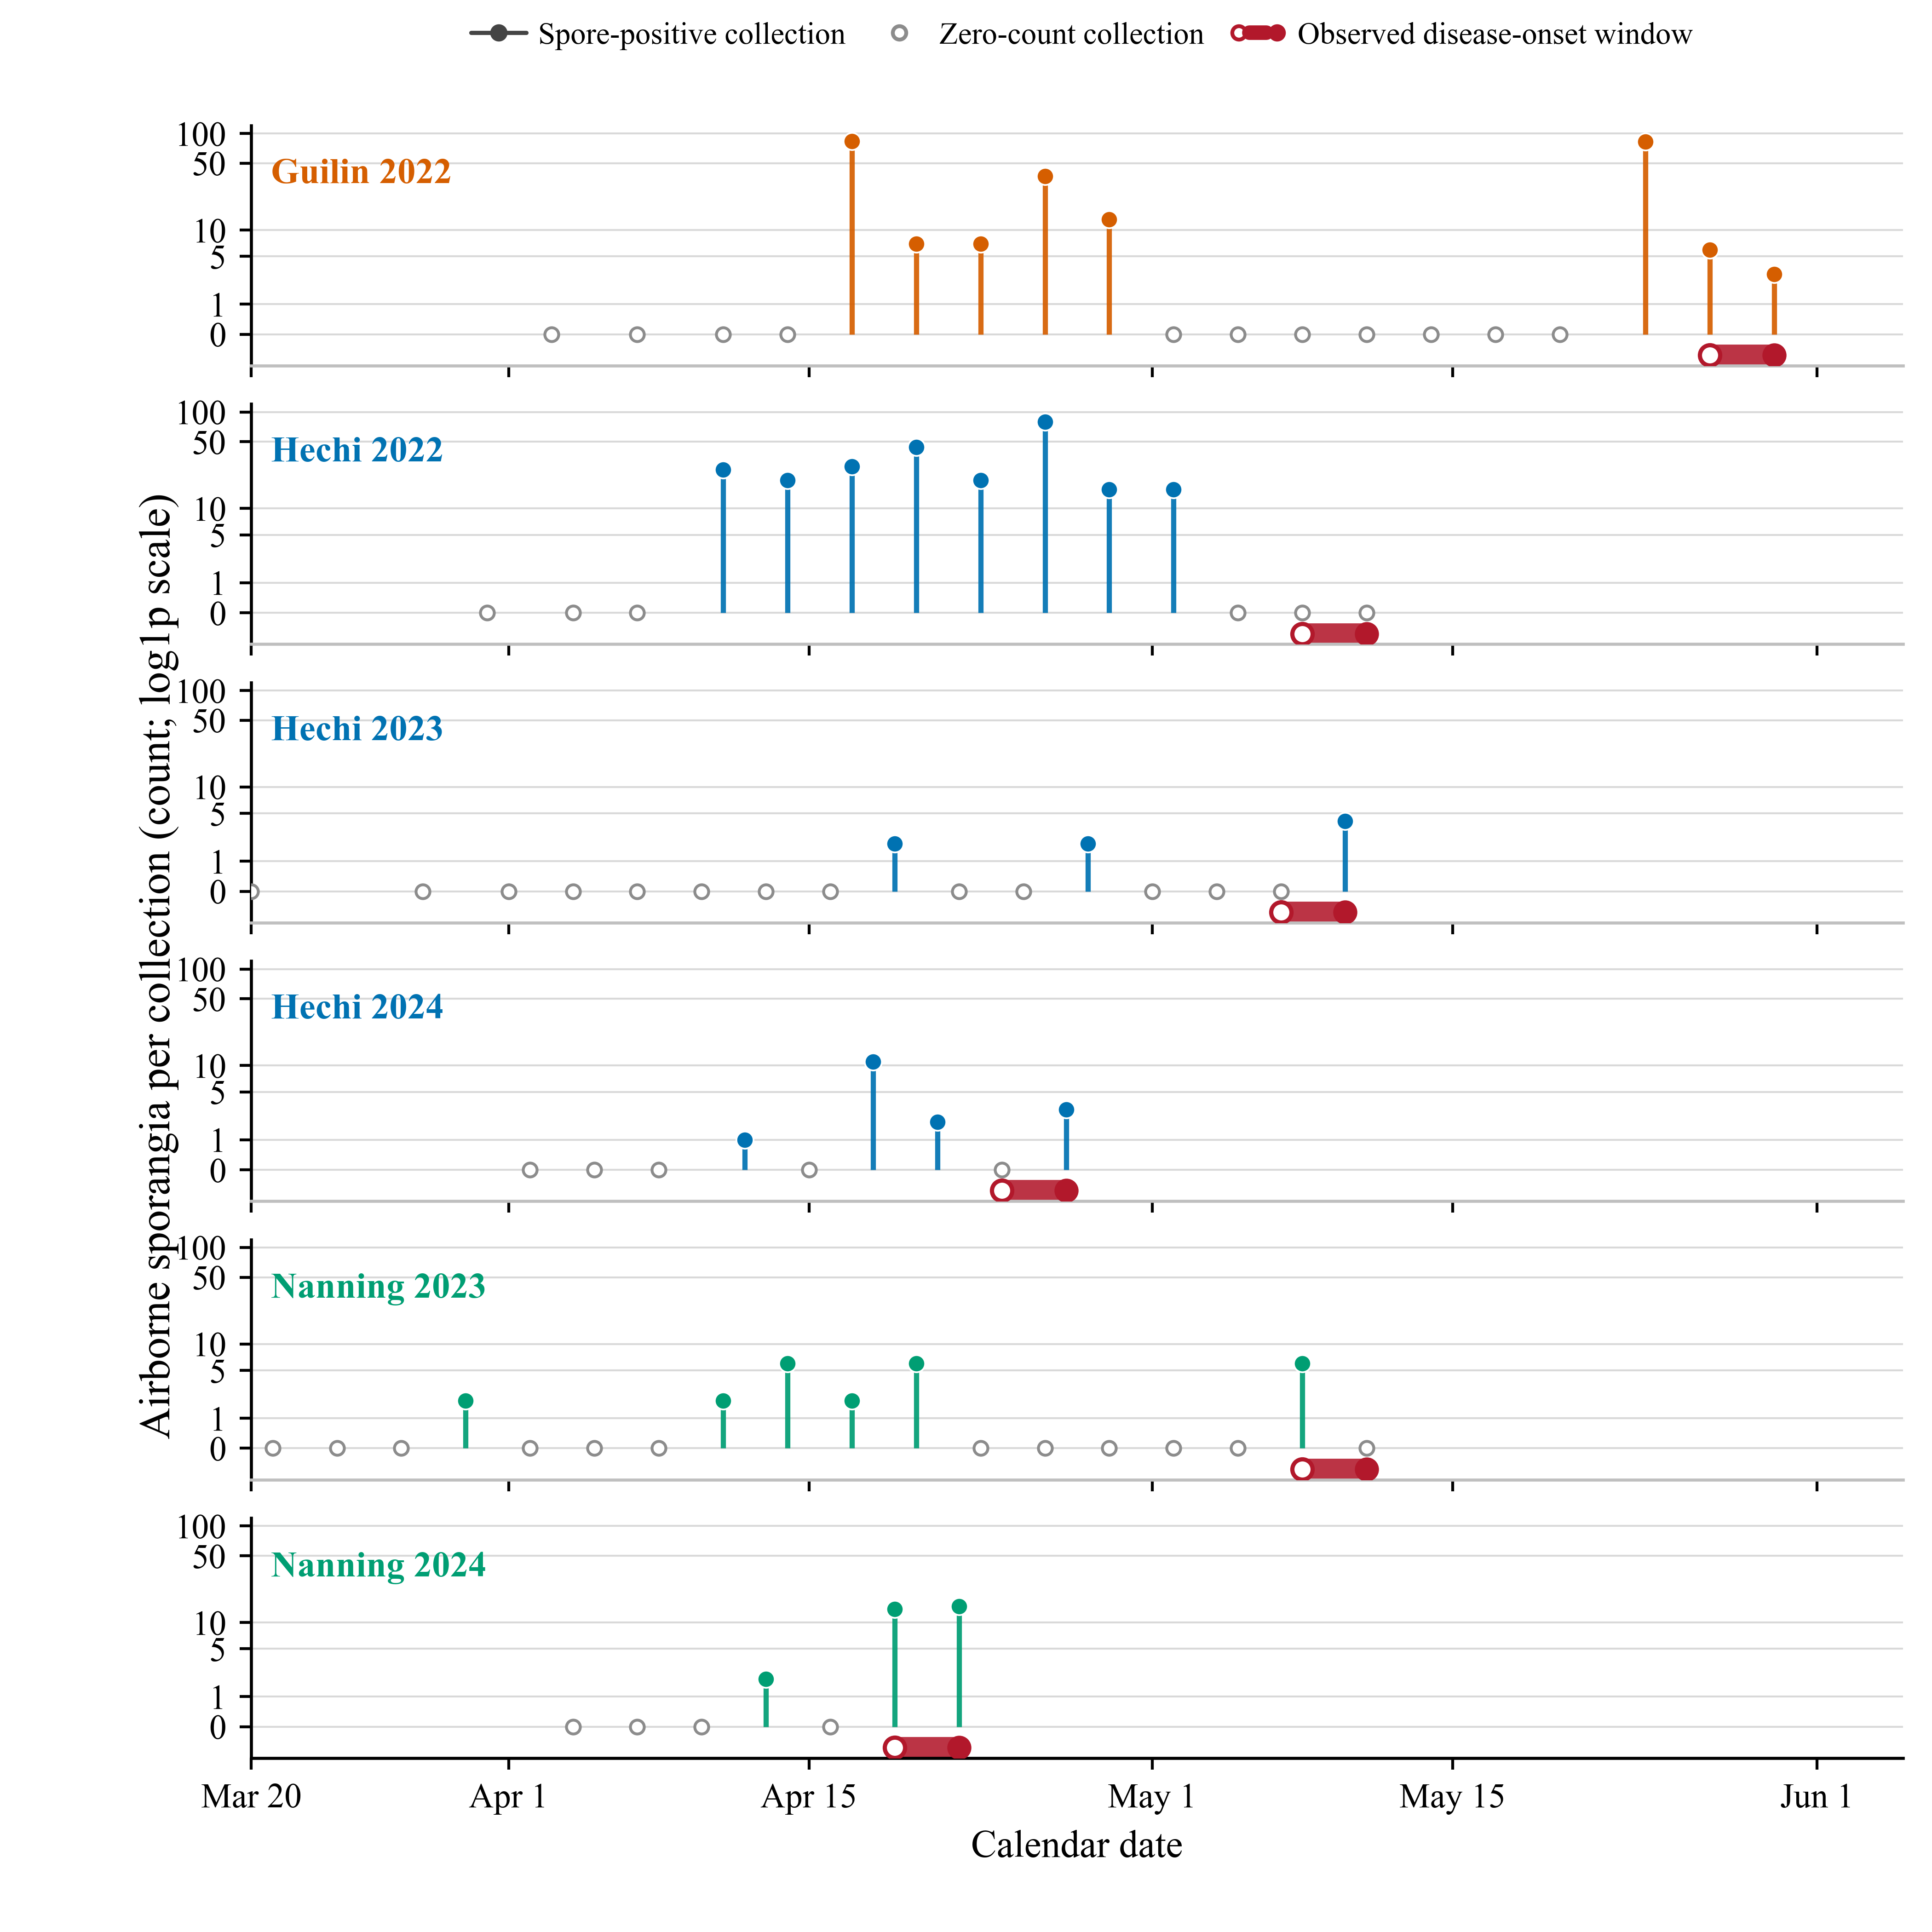
\includegraphics[width=0.95\linewidth]{fig/figure_08.png}
\caption{Experimental observations from Guangxi. Spore-positive and
zero-count collections are shown on a common calendar axis; red bars denote
disease-onset windows between the last negative and first positive
assessments.}
\label{_Ref212492136}
\end{figure}

\subsection{Sensitivity analysis}\label{sensitivity-analysis}

At \(N=1024\), the total-order sensitivity ranking across six site--years
was EDR > SRH > WTH > HWR > IDH > MMH
(\hyperref[_Ref222510092]{Fig 9}). EDR dominated the variation in the
censored mean first symptom-onset day, with \(S_1=0.740\) and
\(S_T=0.817\). Total-order indices were 0.097 for SRH, 0.093 for WTH,
0.087 for HWR, 0.020 for IDH and 0.009 for MMH. Across \(N=256\), 512
and 1024, EDR remained dominant (\(S_T=0.795\)--0.832) and SRH ranked
second. WTH and HWR exchanged ranks, while IDH and MMH consistently had
smaller effects. The overlapping 95\% confidence intervals for SRH, WTH
and HWR indicate that their relative ordering was less clearly resolved
than EDR's dominance.

\begin{figure}[H]
\centering
\includegraphics[width=0.95\linewidth]{fig/figure_09.png}
\caption{Sobol sensitivity of six FSIM parameters for the censored mean
first symptom-onset day across six site--years. (a) First-order (\(S_1\)) and total-order
(\(S_T\)) indices at \(N=1024\); (b) total-order indices across
\(N=256\), 512, and 1024. Error bars show 95\% bootstrap confidence intervals.
Parameter abbreviations: EDR = effective
deposition rainfall threshold; SRH = sporulation relative-humidity
threshold; MMH = minimum moist-hour threshold; HWR = heavy-rain wash-off
threshold; IDH = infection degree-hour threshold; WTH = minimum wind-speed
threshold.}
\label{_Ref222510092}
\end{figure}

\subsection{Model performance}\label{model-performance}

FSIM had a training-set MAE of 5.67 days and RMSE of 7.18 days, and a
validation-set MAE of 5.67 days and RMSE of 7.26 days
(\hyperref[fig:fsim-error-metrics]{Fig 10}).

FSIM-S had a training-set MAE of 3.83 days and RMSE of 5.99 days, and a
validation-set MAE of 3.83 days and RMSE of 6.18 days. Relative to FSIM,
MAE decreased by 32.4\% in both sets; RMSE decreased by 16.6\% in the
training set and 14.9\% in the validation set.

From FSIM to FSIM-S, the site--year errors changed as follows: Hechi 2024,
0 to 0 days; Hechi 2023, -6 to +4 days; Hechi 2022, -14 to -14 days;
Nanning 2024, +4 to +4 days; Nanning 2023, +2 to +1 days; and Guilin
2022, -8 to 0 days (\hyperref[fig:fsim-site-year-errors]{Fig 11}). Zero
error occurred for Hechi 2024 under both models and for Guilin 2022 under
FSIM-S. The largest error magnitude was 14 days in Hechi 2022 and remained
unchanged between models.

\begin{figure}[H]
\centering
\includegraphics[width=0.95\linewidth]{fig/figure_10.png}
\caption{Aggregate first symptom-onset errors for FSIM and FSIM-S. (a) Mean
absolute error (MAE); (b) root mean square error (RMSE). Training values are
means across six outer folds; validation values summarize the six held-out
predictions. Error bars indicate $\pm$ one bootstrap standard error from
site--year resampling with fitted models held fixed. Values are in days.}
\label{fig:fsim-error-metrics}
\end{figure}

\begin{figure}[H]
\centering
\includegraphics[width=0.95\linewidth]{fig/figure_11.png}
\caption{Site--year interval-based errors in first symptom-onset timing
for FSIM and FSIM-S. The shaded region indicates signed distances between
the simulated and observed windows within $\pm 7$ days; overlapping
windows have zero error.}
\label{fig:fsim-site-year-errors}
\end{figure}

\subsection{Spatial distribution of first symptom onset across Guangxi
(2000--2024)}\label{spatial-distribution-of-first-symptom-onset-across-guangxi-2000-2024}

During 2000--2024, mean spring temperature was generally higher in
southern than northern Guangxi. Cumulative spring precipitation was
higher in the east, particularly the northeast, and lower in the west.
Nighttime high-humidity duration was generally longer in the southeast
and shorter in the northwest
(\hyperref[fig:spring-weather-background]{Fig 12a--c}).

Across Guangxi, the grid-cell mean first symptom-window midpoints for
2000--2024 averaged DOY 130.4 under the table-grape scenario and DOY 136.3
under the wine-grape scenario, a difference of 5.9 days
(\hyperref[_Ref223011563]{Fig 13a,b}). Both scenarios showed earlier
onset in eastern and southeastern Guangxi and later onset in western
Guangxi, particularly the northwest.

The distribution of grid-cell mean onset dates was shifted towards later
dates under the wine-grape scenario. The most frequent interval was DOY
120--130 for table grapes and DOY 130--140 for wine grapes
(\hyperref[_Ref223011563]{Fig 13c,d}). Annual regional mean symptom-window
midpoints ranged from DOY 115.7 to 145.6 for table grapes and from DOY 122.8
to 147.8 for wine grapes (Supplementary Figs S2 and S3).

\begin{figure}[H]
\centering
\includegraphics[width=0.95\linewidth]{fig/figure_12.png}
\caption{Spring meteorological conditions in Guangxi during 2000--2024
(March--May). (a--c) Grid-cell means for temperature, cumulative
precipitation and nighttime high-humidity duration (relative humidity
$\geq85\%$; 20:00--07:59 local time). (d--f) Annual regional grid means;
shading indicates spatial 25th--75th percentile ranges and dashed lines
indicate descriptive linear trends.}
\label{fig:spring-weather-background}
\end{figure}

\begin{figure}[H]
\centering
\includegraphics[width=0.95\linewidth]{fig/figure_13.png}
\caption{Mean first symptom-window midpoint (day of year, DOY) per grid cell
in Guangxi during 2000--2024 under the table- and wine-grape scenarios.}
\label{_Ref223011563}
\end{figure}

\subsection{Regional potential for fungicide savings
(2000--2024)}\label{regional-disease-management-implications-2000-2024}

Across Guangxi, the grid-cell mean potential fungicide savings for
2000--2024 averaged approximately 3.5 applications per season under the
table-grape scenario and 4.0 under the wine-grape scenario, a difference
of 0.5 applications (\hyperref[_Ref223012659]{Fig 14a,b}). Both scenarios
showed higher saving potential in western Guangxi, particularly the
northwest, and lower potential in eastern and southeastern Guangxi.

The distribution of grid-cell mean savings was shifted towards higher values
under the wine-grape scenario. The most frequent category was centred on
three applications for table grapes and four applications for wine grapes
(\hyperref[_Ref223012659]{Fig 14c,d}). Annual regional mean potentially
avoidable applications ranged from 2.30 to 4.82 under the table-grape
scenario and from 2.72 to 5.17 under the wine-grape scenario (Supplementary
Figs S4 and S5).

\begin{figure}[H]
\centering
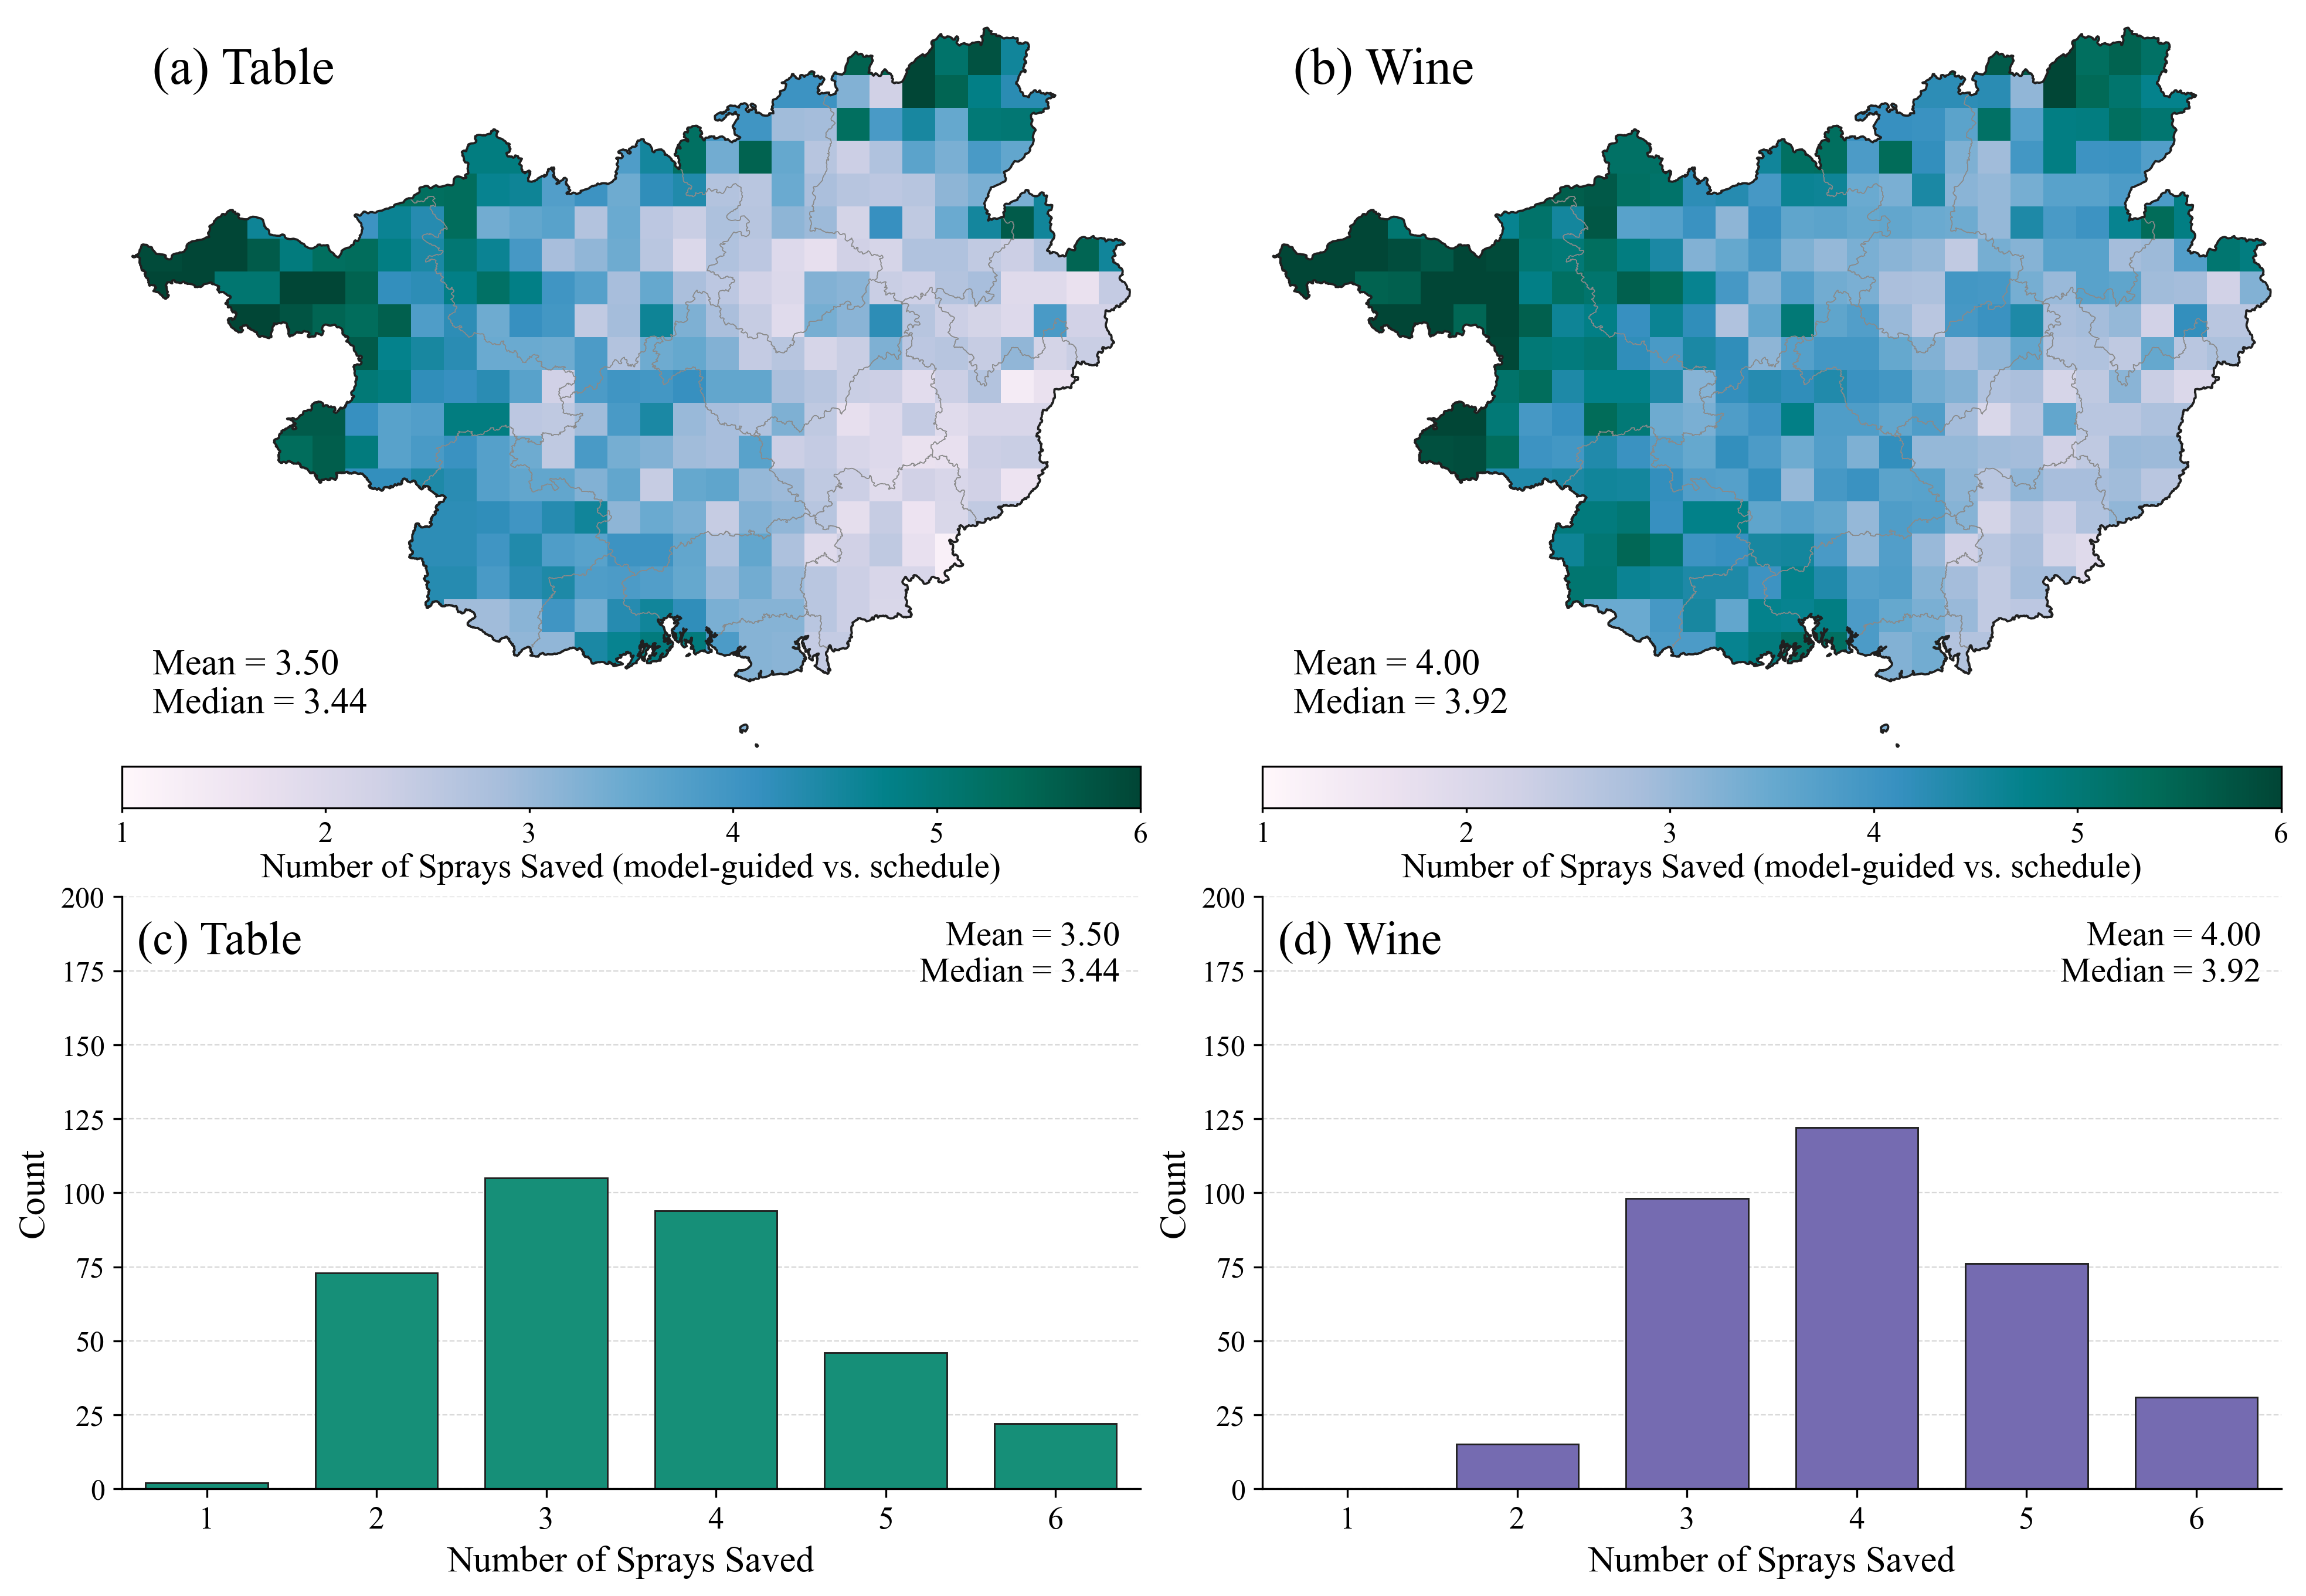
\includegraphics[width=0.95\linewidth]{fig/figure_14.png}
\caption{Mean potential fungicide savings (applications per season) per
grid cell in Guangxi during 2000--2024 under the table- and wine-grape
scenarios. Note: The display range is restricted to 1--6 applications.
Eight table-grape grids and 16 wine-grape grids exceed six applications
and are treated as outlying events; their values beyond six are not
displayed. Figure statistics use values bounded to the display range;
the regional means reported in the text include all original values.}
\label{_Ref223012659}
\end{figure}



\section{DISCUSSION}\label{discussion}

\subsection{Airborne inoculum and first seasonal symptom onset under
double cropping}\label{inoculum-dynamics-and-the-drivers-of-first-seasonal-symptom-onset}

In temperate vineyards, winter dormancy interrupts the availability of green
host tissue, and overwintered oospores provide an important source of
initial inoculum.\textsuperscript{4} In subtropical double-cropping regions,
however, successive production cycles can maintain green tissues in
neighbouring vineyards even when an individual vineyard undergoes leaf fall.
This can allow input of asexually produced sporangia before lesions appear
in the new growing season, consistent with the importance of asexual
infection reported in warm viticultural regions.\textsuperscript{13,15}
Sporangia were captured before the first symptom-positive assessment in all
six site--years (\hyperref[_Ref212492136]{Fig 8}), confirming the widespread
occurrence of external sporangial input across the monitored site-years.
However, this study did not trace the source vineyards of the captured
sporangia, and a potential contribution from oospores cannot be entirely
excluded. A limited role for oospores under these conditions remains
possible, given evidence of their formation and germination in southern
Brazil.\textsuperscript{28}

Earlier sporangial detection did not consistently precede earlier disease
onset. Nanning 2023 had earlier capture but later symptoms than Nanning
2024, with detection-to-assessment intervals of 42 and 9 days, respectively;
Guilin 2022 showed a 43-day interval. In Hechi, similar symptom dates in
2022 and 2023 followed different capture timing and counts, whereas similar
first capture dates in 2022 and 2024 preceded symptom assessments two weeks
apart. These contrasts indicate that neither first detection nor maximum
captured count alone can explain symptom onset; interpretation must also
account for weather conditions and host susceptibility, consistent with the
classical disease triangle framework.\textsuperscript{6}

\subsection{Model performance and improvement}\label{model-enhancement}

FSIM achieved good predictive performance, with a cross-validated mean
absolute error of 5.67 d. Incorporating spore-pressure dynamics into FSIM-S
further reduced the error to 3.83 d, a reduction of 32.4\%
(\hyperref[fig:fsim-error-metrics]{Fig 10}). Because both models retain the
same infection-to-symptom core framework, these results indicate that
inoculum availability carries information beyond meteorological suitability
alone and can improve predictive performance.\textsuperscript{9}

The main methodological advance is the representation of seasonal
initiation when the inoculum source is not synchronized with the local
crop cycle. Models beginning with germinating oospores or visible lesions
encode different starting conditions,\textsuperscript{8,10} whereas FSIM
permits recurrent sporangial exposure before symptoms appear in the
target vineyard. Tracking each cohort through attached survival,
dispersal, airborne survival and deposition preserves the distinction
between inoculum supply and successful infection. FSIM-S then constrains
supply at cohort generation rather than shifting symptom dates after
simulation. This structure gives the monitoring signal an explicit
biological role and retains weather-dependent infection and incubation
as separate filters. Its value in double-cropping systems is therefore
the ability to represent a regional inoculum supply that may persist
while susceptibility develops anew within an individual vineyard.

The error pattern indicates that observation constraints reduce some
timing mismatches without resolving all causes of premature onset.
Validation RMSE decreased by 14.9\%, less than the 32.4\% decrease in MAE,
and the 14-day early error in Hechi 2022 persisted. The remaining large
error warrants targeted examination of inoculum viability, local wetness
and host susceptibility, rather than assuming that more sporangial
detections necessarily improve prediction. Furthermore, the three-day
assessment schedule sets the resolution of the observed onset windows:
zero interval error establishes temporal compatibility, not exact daily
agreement. Prospective tests should therefore pair spore monitoring with
direct leaf-wetness measurements and frequent symptom assessments to
determine whether the improvement reflects better identification of
infectious exposure and remains useful at the timescale of management
decisions.

The distinction between airborne detection and effective inoculum is central
to interpreting this gain. Brischetto et al.\textsuperscript{9} found that
sporangium counts adjusted for weather-dependent survival were more closely
associated with infection than total captured counts, and were particularly
useful for identifying periods without infection. Thus, monitoring is most
informative when interpreted together with the conditions governing survival
and infection. In FSIM-S, the suppression associated with zero captures and
the increase associated with positive spore pressure provide complementary
constraints on inoculum availability, while subsequent biological processes
remain weather dependent. These results demonstrate the value of deploying
spore traps and maintaining continuous monitoring to further refine the
model for early-season disease prevention.\textsuperscript{9,29} However,
zero captures indicate non-detection rather than confirmed absence, and
captured sporangia are not necessarily viable. Relative pressure derived
from passive traps should therefore not be interpreted as an absolute
concentration of infectious inoculum or assigned thresholds established with
volumetric samplers.

Recent developments strengthen the case for connecting sporangium
monitoring with disease models. Muthukumar et al.\textsuperscript{29} detected
airborne \emph{P. viticola} using impaction traps and qPCR 10--14 days
before visible symptoms. Malvessi Cattani et al.\textsuperscript{30} used automated
air-flow cytometry, although agreement with reference measurements was
weaker during early leaf development and flowering than later in the
season. These findings highlight both the opportunity for earlier
biological information and the difficulty of measuring sparse
early-season inoculum. FSIM-S connects this measurable exposure signal
with survival, dispersal, deposition, infection and symptom development,
adding observation-based constraints on inoculum availability to predict
first onset in subtropical double-cropping vineyards.

\subsection{Regional implications for disease management}
\label{regional-implications-for-disease-management}

The mean east--west contrast in symptom onset under both cultivation
scenarios (\hyperref[_Ref223011563]{Fig 13}) indicates that a single
province-wide onset date would obscure locally different disease
trajectories. Earlier eastern and southeastern onset broadly coincided with
greater spring rainfall and longer nighttime high-humidity duration
(\hyperref[fig:spring-weather-background]{Fig 12a--c}). Humid nights support
recurrent sporulation and sporangial survival, while suitable rain events
enable deposition and subsequent infection.\textsuperscript{8,10} Lower
western rainfall may delay the coincidence of viable inoculum, leaf wetness
and susceptible host tissue. These results show that FSIM can use hourly
weather data and host development information to simulate differences in
symptom onset across space and time, indicating potential for broader
application and further validation.

These spatial patterns are best interpreted as the outcome of sequential
biological filters rather than a response to a single climatic variable. The
effective deposition rainfall threshold dominated the sensitivity analysis,
while the sporulation humidity, wind-speed and heavy-rain wash-off
thresholds had smaller total-order effects (\hyperref[_Ref222510092]{Fig
9}), highlighting the roles of inoculum deposition, humid-night sporulation
and dispersal in simulated onset. Within the model, rainfall can enable
deposition or remove airborne cohorts under the assumed wash-off rule;
seasonal totals alone therefore cannot identify individual infection
opportunities. Similarly, higher southern temperatures need not produce the
earliest symptoms if moisture or host susceptibility is limiting. These
mechanisms provide a coherent explanation for the spatial contrasts in
symptom onset, indicating that FSIM can effectively capture the effects of
spatiotemporal variation in influential variables.

Annual reconstructions show that the timing and spatial extent of early
symptom expression vary among seasons under both cultivation scenarios
(Supplementary Figs S2 and S3). The long-term mean maps therefore provide a
regional background for surveillance, while seasonal decisions also depend
on the timing of individual weather events and host development. The
interannual meteorological variability in Fig 12d--f provides context for
these differences, although the contributions of individual drivers were not
separated. Because the process framework is evaluated hourly at each grid,
current-season weather and meteorological forecasts could support repeated
updates of regional onset windows and season-specific surveillance, subject
to forecast uncertainty and operational evaluation.

The spatial correspondence between later symptom onset and greater potential
spray savings has a clear disease-management basis. Compared with a fixed
calendar-based fungicide programme, later symptom onset in western and
northwestern Guangxi leaves more early applications potentially avoidable
(\hyperref[_Ref223012659]{Fig 14}). Full-grid means of 3.5 and 4.0
applications are scenario estimates, not measured reductions or
vineyard-area-weighted totals. The annual maps further show that the spatial
extent of high saving potential changes among years (Supplementary Figs S4
and S5); the multi-year means should therefore not be treated as fixed
annual reduction targets. Together, these results highlight FSIM's potential
to guide reductions in fungicide applications under regional cultivation
scenarios.

For the grape industry, this spatial and annual differentiation could
support earlier surveillance and protection readiness in zones with earlier
onset, while identifying where routine early applications warrant closer
reassessment. Regional warning services could combine a common
weather-driven framework with local observations to prioritize scouting,
technical advice and application resources. The practical aim is to
concentrate protection around locally relevant infection periods while
limiting poorly timed inputs, rather than applying a uniform reduction
target across the province.

\subsection{Limitations and future
directions}\label{limitations-and-future-directions}

This initial framework relies on observations from two commercial
vineyards and one experimental vineyard over three growing seasons.
Additional regions, cultivars and management systems would broaden
calibration and evaluation. Guilin 2022, with relatively low April
humidity and uneven rainfall, illustrates conditions that may delay or
suppress infection establishment and help test whether the model
distinguishes inoculum presence from conditions permitting infection.

FSIM-S uses a deterministic structure coupling weather and spore-pressure
dynamics, favouring stability, interpretability and transparent
biological assumptions. Probabilistic extensions could quantify
uncertainty from rainfall variability, spore sampling error and
fine-scale atmospheric heterogeneity. The regional analysis also
represents scenarios rather than vineyard-specific operational risk,
using simplified vineyard, canopy and cultivar assumptions. Vineyard
land-use layers, cultivar distribution, remote-sensing information and
canopy microclimate observations would support more spatially resolved
deployment.

\section{CONCLUSION}\label{conclusion}

FSIM provides a process-based framework for predicting first-season
grapevine downy mildew symptom onset under subtropical double cropping,
linking airborne sporangial inoculum, weather and host development.
Across six site--years in Guangxi, its validation mean absolute error was
5.67 days. Incorporating observed spore pressure in FSIM-S reduced this
error to 3.83 days, a 32.4\% improvement, demonstrating the additional
predictive value of spore monitoring within the mechanistic framework.

Regional FSIM simulations for 2000--2024 showed earlier mean symptom onset
in eastern and southeastern Guangxi and later onset in western and
northwestern areas. Mean onset was 5.9 days later in the wine-grape scenario
than in the table-grape scenario. Relative to the reference spray
programme, estimated potential savings averaged 3.5 early applications per
season for table grapes and 4.0 for wine grapes. These spatial and
phenological differences support adapting early-season protection to local
disease risk and crop development. Prospective field trials are needed to
establish whether the estimated savings can be achieved while maintaining
disease control. Together, these findings provide a basis for risk-based
preventive programmes that use weather and phenology, supplemented by
spore monitoring where available, to reduce unnecessary fungicide use in
subtropical double-cropping vineyards.

\section*{Acknowledgements}\label{acknowledgements}

This work was funded by Guangxi Key R\&D Program Project (Grant No. Gui
Ke AB24010121, AB21076001) and the Key Research and Development Program
of Shaanxi (Grant No. 2023-ZDLNY-64). We gratefully acknowledge Mr. Yunlong Chen and Mr.
Yaokang Liang, local growers in Guilin and Hechi, for their valuable
assistance in fieldwork.

\section*{Conflict of Interest}\label{declaration-of-competing-interest}

The authors declare that they have no known competing financial
interests or personal relationships that could have appeared to
influence the work reported in this paper.

\section*{CRediT authorship contribution
statement}\label{credit-authorship-contribution-statement}

Linjia Yao: Investigation, Writing -- original draft, Visualization,
Software, Methodology, Formal analysis, Conceptualization. Bin Chen:
Investigation, Writing -- original draft, Formal analysis, Writing
-- review \& editing. Vittorio Rossi: Formal analysis, Writing -- review \&
editing. Ling Yin: Funding acquisition, Writing -- review \& editing.
Shumei Wei: Investigation. Qi Tian: Investigation. Changqing Yan:
Writing -- review \& editing. Hui Wang: Writing -- review \& editing.
Antonio Fernandes Nogueira Júnior: Writing -- review \& editing. Yu Huang:
Investigation. Qiang Yu: Conceptualization, Supervision. Junjie Qu:
Funding acquisition. Gang Zhao: Software, Methodology,
Conceptualization, Supervision.

\section*{Data Availability}\label{data-availability}

The model structure, code, and data supporting the findings of this study
are available from the corresponding author upon reasonable request
(\ul{gang.zhao@nwafu.edu.cn (Gang Zhao)}).

\section*{Supporting information}\label{supporting-information}

Supporting information may be found in the online version of this article.

\section*{References}\label{references}

1 Koledenkova K, Esmaeel Q, Jacquard C, Nowak J, Clément C and Ait Barka E, \emph{Plasmopara viticola}, the causal agent of downy mildew of grapevine: From its taxonomy to disease management. \emph{Front Microbiol} \textbf{13}:889472. \url{https://doi.org/10.3389/fmicb.2022.889472} (2022).

2 Peng J, Wang X, Wang H, Li X, Zhang Q, Wang M et al., Advances in understanding grapevine downy mildew: From pathogen infection to disease management. \emph{Mol Plant Pathol} \textbf{25}:e13401. \url{https://doi.org/10.1111/mpp.13401} (2024).

3 Nogueira Júnior AF, Ribeiro RV, Marcos FCC and Amorim L, Virtual lesions and photosynthetic damage caused by \emph{Plasmopara viticola} in \emph{Vitis labrusca}. \emph{Eur J Plant Pathol} \textbf{155}:545--555. \url{https://doi.org/10.1007/s10658-019-01791-2} (2019).

4 Gessler C, Pertot I and Perazzolli M, \emph{Plasmopara viticola}: A review of knowledge on downy mildew of grapevine and effective disease management. \emph{Phytopathol Mediterr} \textbf{50}:3--44. \url{https://www.jstor.org/stable/26458675} (2011).

5 Caffi T, Rossi V and Bugiani R, Evaluation of a warning system for controlling primary infections of grapevine downy mildew. \emph{Plant Dis} \textbf{94}:709--716. \url{https://doi.org/10.1094/PDIS-94-6-0709} (2010).

6 Scholthof K-BG, The disease triangle: pathogens, the environment and society. \emph{Nat Rev Microbiol} \textbf{5}:152--156. \url{https://doi.org/10.1038/nrmicro1596} (2007).

7 Caffi T, Rossi V, Cossu A and Fronteddu F, Empirical vs. mechanistic models for primary infections of \emph{Plasmopara viticola}. \emph{EPPO Bull} \textbf{37}:261--271. \url{https://doi.org/10.1111/j.1365-2338.2007.01120.x} (2007).

8 Rossi V, Caffi T, Giosuè S and Bugiani R, A mechanistic model simulating primary infections of downy mildew in grapevine. \emph{Ecol Model} \textbf{212}:480--491. \url{https://doi.org/10.1016/j.ecolmodel.2007.10.046} (2008).

9 Brischetto C, Bove F, Languasco L and Rossi V, Can spore sampler data be used to predict \emph{Plasmopara viticola} infection in vineyards? \emph{Front Plant Sci} \textbf{11}:1187. \url{https://doi.org/10.3389/fpls.2020.01187} (2020).

10 Brischetto C, Bove F, Fedele G and Rossi V, A weather-driven model for predicting infections of grapevines by sporangia of \emph{Plasmopara viticola}. \emph{Front Plant Sci} \textbf{12}:636607. \url{https://doi.org/10.3389/fpls.2021.636607} (2021).

11 Chen W-K, Bai X-J, Cao M-M, Cheng G, Cao X-J, Guo R-R et al., Dissecting the variations of ripening progression and flavonoid metabolism in grape berries grown under double cropping system. \emph{Front Plant Sci} \textbf{8}:1912. \url{https://doi.org/10.3389/fpls.2017.01912} (2017).

12 Lu H-C, Chen W-K, Wang Y, Bai X-J, Cheng G, Duan C-Q et al., Effect of the seasonal climatic variations on the accumulation of fruit volatiles in four grape varieties under the double cropping system. \emph{Front Plant Sci} \textbf{12}:809558. \url{https://doi.org/10.3389/fpls.2021.809558} (2022).

13 Camargo MP, Hong CF, Amorim L and Scherm H, Cryptic species and population genetic structure of \emph{Plasmopara viticola} in São Paulo State, Brazil. \emph{Plant Pathol} \textbf{68}:719--726. \url{https://doi.org/10.1111/ppa.12993} (2019).

14 Vercesi A, Toffolatti SL, Zocchi G, Guglielmann R and Ironi L, A new approach to modelling the dynamics of oospore germination in \emph{Plasmopara viticola}. \emph{Eur J Plant Pathol} \textbf{128}:113--126. \url{https://doi.org/10.1007/s10658-010-9635-8} (2010).

15 Koopman T, Linde CC, Fourie PH and McLeod A, Population genetic structure of \emph{Plasmopara viticola} in the Western Cape Province of South Africa. \emph{Mol Plant Pathol} \textbf{8}:723--736. \url{https://doi.org/10.1111/j.1364-3703.2007.00429.x} (2007).

16 Killigrew BX, Sivasithamparam K and Scott ES, Absence of oospores of downy mildew of grape caused by \emph{Plasmopara viticola} as the source of primary inoculum in most Western Australian vineyards. \emph{Plant Dis} \textbf{89}:777. \url{https://doi.org/10.1094/PD-89-0777C} (2005).

17 Lorenz DH, Eichhorn KW, Bleiholder H, Klose R, Meier U and Weber E, Growth stages of the grapevine: Phenological growth stages of the grapevine (\emph{Vitis vinifera} L. ssp. vinifera)---Codes and descriptions according to the extended BBCH scale. \emph{Aust J Grape Wine Res} \textbf{1}:100--103. \url{https://doi.org/10.1111/j.1755-0238.1995.tb00085.x} (1995).

18 Hersbach H, Bell B, Berrisford P, Hirahara S, Horányi A, Muñoz-Sabater J et al., The ERA5 global reanalysis. \emph{Q J R Meteorol Soc} \textbf{146}:1999--2049. \url{https://doi.org/10.1002/qj.3803} (2020).

19 Huber L and Gillespie TJ, Modeling leaf wetness in relation to plant disease epidemiology. \emph{Annu Rev Phytopathol} \textbf{30}:553--577. \url{https://doi.org/10.1146/annurev.py.30.090192.003005} (1992).

20 Sobol IM, Global sensitivity indices for nonlinear mathematical models and their Monte Carlo estimates. \emph{Math Comput Simul} \textbf{55}:271--280. \url{https://doi.org/10.1016/S0378-4754(00)00270-6} (2001).

21 Wang H, Zhang W, Bregaglio S, Yu S, Li X, Li Y et al., Adoption of Sobol's analysis method improved the application of a coupled primary and secondary infection grape downy mildew model in northern China. \emph{Comput Electron Agric} \textbf{199}:107154. \url{https://doi.org/10.1016/j.compag.2022.107154} (2022).

22 Iooss B and Lemaître P, A review on global sensitivity analysis methods, in \emph{Uncertainty Management in Simulation-Optimization of Complex Systems}, ed. by Dellino G and Meloni C. Springer, Boston, MA, pp. 101--122. \url{https://doi.org/10.1007/978-1-4899-7547-8\_5} (2015).

23 Kennelly MM, Gadoury DM, Wilcox WF, Magarey PA and Seem RC, Seasonal development of ontogenic resistance to downy mildew in grape berries and rachises. \emph{Phytopathology} \textbf{95}:1445--1452. \url{https://doi.org/10.1094/PHYTO-95-1445} (2005).

24 Reuveni M, Relationships between leaf age, peroxidase and \(\beta\)-1,3-glucanase activity, and resistance to downy mildew in grapevines. \emph{J Phytopathol} \textbf{146}:525--530. \url{https://doi.org/10.1111/j.1439-0434.1998.tb04615.x} (1998).

25 Karabektaşoğlu Ş, Köse B and Svyantek A, Investigation of the phenological and climate indices of some table and wine grapes and their growing status in the Samsun-Bafra Plain (Türkiye). \emph{Anadolu J Agric Sci} \textbf{39}:143--162. \url{https://doi.org/10.7161/omuanajas.1394670} (2024).

26 Hu M and Fiola J, Downy mildew management. University of Maryland Extension. \url{https://extension.umd.edu/resource/downy-mildew-management} (2024) [accessed 9 October 2026].

27 Wang X, Li H and García De Cortázar Atauri I, Assessing grapevine phenological models under Chinese climatic conditions. \emph{OENO One} \textbf{54}:637--656. \url{https://doi.org/10.20870/oeno-one.2020.54.3.3195} (2020).

28 Bitencourt C, Perazzoli V, de Freitas FR, Soldi C, da Silva AL and Welter LJ, Sexual reproduction of \emph{Plasmopara viticola} in wine regions of southern Brazil, climatic suitability, oospore formation and germination. \emph{Plant Pathol} \textbf{75}:e70175. \url{https://doi.org/10.1111/ppa.70175} (2026).

29 Muthukumar G, Kamalakannan A, Johnson I, Kamaraj P, Muthuvel I, Varanavasiappan S et al., Early detection and quantification of airborne inocula of \emph{Plasmopara viticola} causing grapevine downy mildew using impaction spore trap. \emph{Physiol Mol Plant Pathol} \textbf{139}:102842. \url{https://doi.org/10.1016/j.pmpp.2025.102842} (2025).

30 Malvessi Cattani A, Zeder Y, Graf E, Schwendimann A, Coronelli R, Smit-Sadki T et al., Automated air-flow cytometry enables real-time monitoring of \emph{Plasmopara viticola} sporangia in vineyards. \emph{Appl Environ Microbiol} \textbf{92}:e02152-25. \url{https://doi.org/10.1128/aem.02152-25} (2026).

\end{document}
